\documentclass[presentation]{beamer}
\usepackage[utf8]{inputenc}
\usepackage[T1]{fontenc}
\usepackage[english]{babel}
\usepackage{lmodern}
\usepackage{amsmath}
\usepackage{amssymb}
\usepackage{amsthm}
\usepackage[superscript]{cite}
\usepackage{nicefrac}
\usepackage{upgreek}
\usepackage{stmaryrd}
\usepackage{tikz}
\usepackage{pgffor}
\usepackage{pgfplots}
\usepackage{graphicx}
\usepackage{caption}
\usepackage{subcaption}
\usepackage{qtree}
\usepackage{dsfont}
\usepackage{eurosym}
\usepackage{tabulary}
\usepackage{setspace}
% \usepackage[colorlinks=true,linkcolor=blue]{hyperref}				% Blaue Links sehen meiner Ansicht nach besser aus als die rot umrandeten Verweise

\usetheme{Madrid}				% Verwende Goettingen für TOC auf jeder Seite, Madrid ohne Navigation
\definecolor{rgbmagenta}{rgb}{1,0,1}
% Kommandos, Operatoren, etc.
\newcommand{\abs}[1]{\lvert#1\rvert}
\newcommand{\norm}[1]{\lVert#1\rVert}
\DeclareMathOperator{\thetafunc}{\uptheta}

% ENDE PRÄAMBEL

\AtBeginSection[]{
	\begin{frame}
		\vfill
		\centering
		\begin{beamercolorbox}[sep=8pt,center,shadow=true,rounded=true]{title}
			\usebeamerfont{title}\insertsectionhead\par%
		\end{beamercolorbox}
		\vfill
	\end{frame}
}

\author{Dominik Blank}
\title{On the influence of morphological operators\\ on testing for a region of interest}
\institute{Georg-August-Universität Göttingen}

\setlength{\parindent}{0pt}
\allowdisplaybreaks

\begin{document}

\begin{frame}
	\maketitle
\end{frame}

\section{Motivation}

\begin{frame}
	\centering
	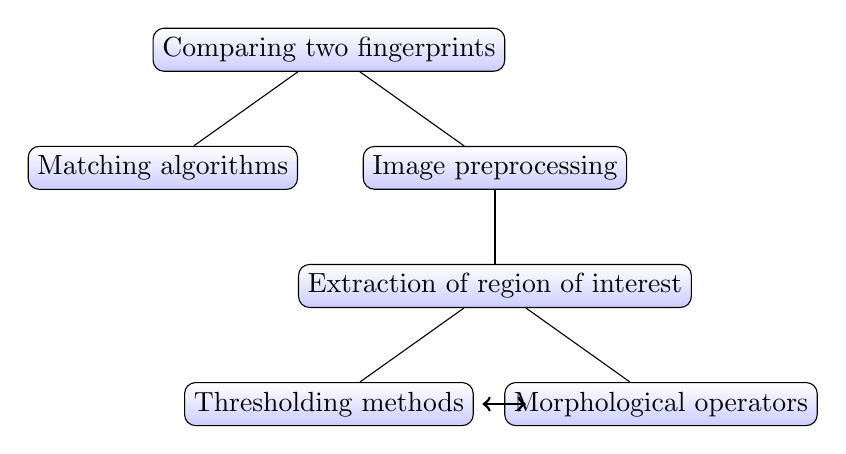
\begin{tikzpicture}[sibling distance=12em, every node/.style = {shape=rectangle, rounded corners,
		draw, align=center, top color=white, bottom color=blue!20}]]
		\node {Comparing two fingerprints}
		child { node {Matching algorithms} }
		child { node {Image preprocessing}
			child { node {Extraction of region of interest}
				child { node {Thresholding methods} }
				child { node {Morphological operators} } } };
		\pause
		\draw [<->, line width=1pt] (1.95, -4.5) -- (2.5, -4.5);
	\end{tikzpicture}
\end{frame}

\begin{frame}
	\begin{figure}
		\centering
		\begin{subfigure}[t]{0.45\linewidth}
			\centering
			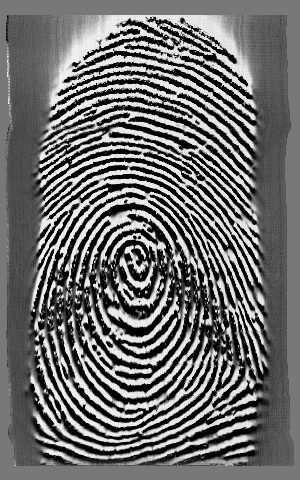
\includegraphics[width=0.7\linewidth]{Thresholding/Fingerprint}
			\caption{Fingerprint}
		\end{subfigure}
		\hfill
		\begin{subfigure}[t]{0.45\linewidth}
			\centering
			
\includegraphics[width=0.7\linewidth]{Thresholding/ROI}
			\caption{Binarized region of interest}
		\end{subfigure}
		\caption{Example of region of interest extraction.}
	\end{figure}
\end{frame}

\begin{frame}
	\begin{block}{Thresholding methods}
		Provide a binarization of the image to categorize pixels into ROI and background.
	\end{block}
	\pause
	\begin{block}{Morphological operators}
		Improve the categorization.
	\end{block}
	\pause
	\begin{alertblock}{Interpretation}
		Interpretation as a statistical test.
		\begin{itemize}
			\item<1-> Falsely classifying a background pixel as foreground $\Leftrightarrow$ Type I error
			\item<2-> Falsely classifying a foreground pixel as background $\Leftrightarrow$ Type II error
			\item<3-> Morphological operators: Lower the amount of the errors in this testing procedure.
		\end{itemize}
	\end{alertblock}
\end{frame}

\begin{frame}
	\begin{beamercolorbox}[sep=8pt,center,shadow=true,rounded=true]{title}
		Goal: Quantify the change of the probabilities of type I and II errors through application of morphological operators \pause \emph{for a specifix pixel}.
	\end{beamercolorbox}
\end{frame}

\begin{frame}
	\begin{itemize}
		\item Assume a simplified model: Rectangular region of interest with a checkerboard pattern surrounded by a constant gray background.
		\begin{itemize}
			\item We can bound the probability of a type I error after thresholding.
			\item The model still exhibits convexity of the ROI and an oscillatory pattern within the ROI, as in a fingerprint image.
		\end{itemize}
		\item Only analyze morphological opening and closing.
	\end{itemize}
\end{frame}

\begin{frame}
	\begin{figure}[h]
		\centering
		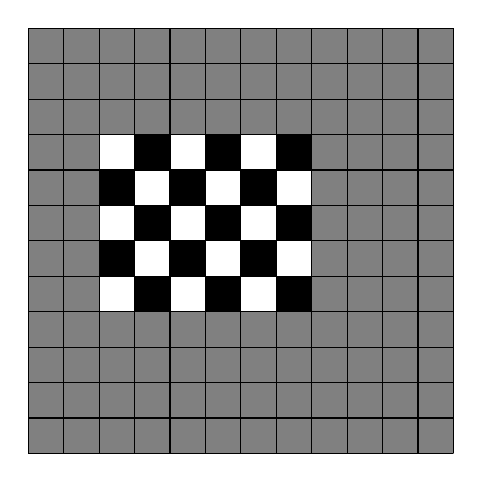
\begin{tikzpicture}[scale=0.45]
			\foreach \i in {-6, ..., 5}
				\foreach \j in {-6, ..., 5}
					\filldraw[gray] (\i, \j) rectangle + (1, 1);
			\foreach \i in {-4, ..., 1}
				\foreach \j in {-2, ..., 2}
				{
					\pgfmathparse{mod(\i+\j, 2) ? "black" : "white"}
					\edef\colour{\pgfmathresult}
					\filldraw[fill=\colour] (\i, \j) rectangle + (1, 1);
				}
			\draw[step=1] (-6, -6) grid (6, 6);
		\end{tikzpicture}
		\caption{Example of an image, that contains a rectangular region of interest with a checkerboard pattern. ($m = 12$, $n = 12$)}
	\end{figure}
\end{frame}

\begin{frame}{Roadmap}
	\tableofcontents
\end{frame}

\section{Thresholding}

\subsection{The statistical model}

\begin{frame}{The statistical model}
	Let $m, n \in \mathbb{N}$ and $\Omega = \left\{ 1, \dots, m \right\} \times  \left\{ 1, \dots, n \right\}$. Assume we are given data
	\begin{equation*}
		F(i, j) = c + V(i, j) + \varepsilon_{i, j}
	\end{equation*}
	\begin{itemize}
		\item $(i, j) \in \Omega$
		\item $c \in \mathbb{R}$ is constant
		\item $V(i, j) \in \{ 0, \pm c \}$
		\item $\varepsilon_{i, j} \sim \mathcal{N}(0, \sigma^2)$ i.i.d. normal distributed random variables
	\end{itemize}
	
	Assumption 1: The image $V$ contains a rectangular region of interest.
	Assumption 2: The ROI has a checkerboard pattern.
\end{frame}

\begin{frame}
	\begin{figure}
		\centering
		\begin{subfigure}[t]{0.45\linewidth}
			\centering
			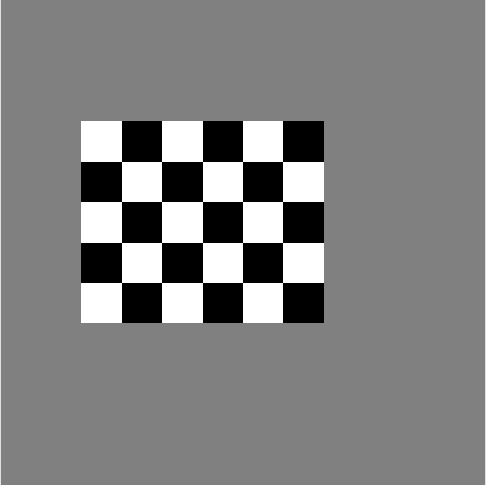
\includegraphics[width=0.9\linewidth]{Thresholding/exampleV}
			\caption{Example of a possible image $V$. ($m = 12$, $n = 12$)}
		\end{subfigure}
		\hfill
		\begin{subfigure}[t]{0.45\linewidth}
			\centering
			
\includegraphics[width=0.9\linewidth]{Thresholding/exampleFsigma50}
			\caption{Example of a possible $F$. Same $V$ as on the left side with noise added. ($\sigma = 50$)}
		\end{subfigure}
	\end{figure}
\end{frame}

\begin{frame}{Simplifications}
	\begin{enumerate}
		\item Assume variance $\sigma$ of the noise terms to be known beforehand.
		\item Ignore the limitations of grayscale images and let the images in our model take all values in the real numbers.
	\end{enumerate}
\end{frame}

\begin{frame}
	\begin{definition}
		Let $m, n \in \mathbb{N}$ and let $V \in \mathbb{R}^{m \times n}$. Let $(i, j) \in \Omega$. The \textit{forward and backward discrete derivative of $V$ evaluated at $(i, j)$} are defined as
		\begin{equation*}
			\Delta^+ V(i, j) =
			\begin{pmatrix}
				V(i + 1, j) - V(i, j) \\
				V(i, j + 1) - V(i, j)
			\end{pmatrix}
			\in \mathbb{R}^2
		\end{equation*}
		and
		\begin{equation*}
			\Delta^- V(i, j) =
			\begin{pmatrix}
				V(i - 1, j) - V(i, j) \\
				V(i, j - 1) - V(i, j)
			\end{pmatrix}
			\in \mathbb{R}^2,
		\end{equation*}
		respectively.
	\end{definition}
\end{frame}

\subsection{Find a statistical test to test for the ROI}

\begin{frame}{Testing for the ROI}
	Observation: Pixel $(i, j)$ being a background pixel is equivalent to $\min \{ \norm{\Delta^+ V(i, j)}, \norm{\Delta^- V(i, j)} \} = 0$.
	
	\begin{block}{The statistical test}
		The null hypothesis, alternative hypothesis and test statistic for our testing procedure are
		\begin{align*}
			H_0(i, j)&: \min \{ \norm{\Delta^+ V(i, j)}, \norm{\Delta^- V(i, j)} \} = 0 \\
			H_1(i, j)&: \min \{ \norm{\Delta^+ V(i, j)}, \norm{\Delta^- V(i, j)} \} \neq 0 \\
			T(i, j) &:= \min \{ \norm{\Delta^+ F(i, j)}, \norm{\Delta^- F(i, j)} \}
		\end{align*}
	\end{block}
\end{frame}

\begin{frame}
	\begin{figure}
		\centering
		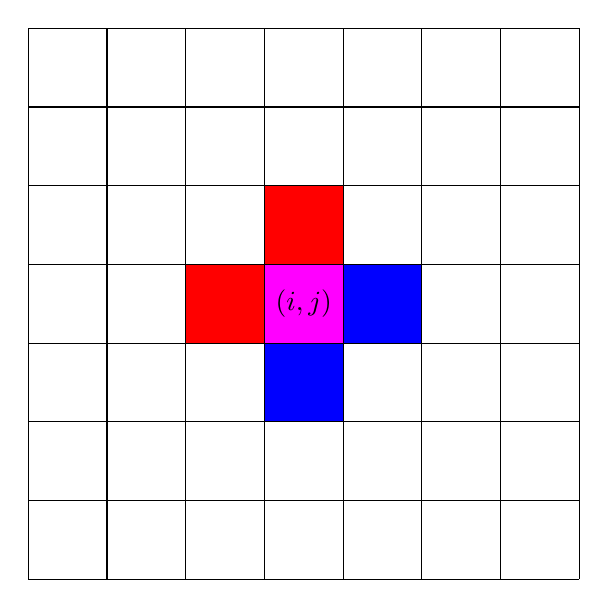
\begin{tikzpicture}
			\foreach \x in {(0, 0), (-1, 0), (0, 1)}
				\filldraw[red] \x rectangle + (1, 1);
			\foreach \x in {(1, 0), (0, -1), (0, 0)}
				\filldraw[blue] \x rectangle + (1, 1);
			\filldraw[rgbmagenta] (0, 0) rectangle + (1, 1);
			\draw[step=1] (-3, -3) grid (4, 4);
			\node at (0.5, 0.5) {$(i, j)$};
		\end{tikzpicture}
		\caption{The random variable $\norm{\Delta^- F(i, j)}$ depends on $(i, j)$ and the red pixels. The random variable $\norm{\Delta^+ F(i, j)}$ depends on $(i, j)$ and the blue pixels.}
	\end{figure}
\end{frame}

\begin{frame}{Notation}
	\begin{tabular}{p{2cm}p{9cm}}
		$\mathcal{V}_c^{m, n}$ & Set of images $V \in \{ 0, \pm c \}^{m \times n}$ that contain a rectangular region of interest with a checkerboard pattern. \\
		$\mathbb{P}_V( \ldots )$ & Probability of an event given a \emph{fixed} image $V$. \\
		$\mathcal{H}_0(i, j)$ & Subset of $\mathcal{V}_c^{m, n}$, such that the null hypothesis at $(i, j)$ is true. \\
		$\mathcal{H}_1(i, j)$ & Subset of $\mathcal{V}_c^{m, n}$, such that the alternative hypothesis at $(i, j)$ is true. \\
		$\Delta^+, \Delta^-$ & Forward and backward discrete derivative operator. \\
		$\norm{.}$ & $\ell^2$-norm \\
	\end{tabular}
\end{frame}

\subsection{Bound for the probability of a type I error}

\begin{frame}{Bound for the probability of a type I error}
	\begin{beamercolorbox}[sep=8pt,center,shadow=true,rounded=true]{title}
		Goal: Given a statistical significance $\alpha$, find a threshold $t_\alpha$, such that
		\begin{equation*}
			\mathbb{P}_V( T(i, j) \geq t_\alpha ) \leq \alpha
		\end{equation*}
		for every $V \in \mathcal{H}_0(i, j)$.
	\end{beamercolorbox}
\end{frame}

\begin{frame}{Bound for the probability of a type I error - Step 0}
	Define
	\begin{align*}
		\mathcal{H}_0^+(i, j) &:= \left\{ V \in \mathcal{V}_c^{m, n} \mid \norm{\Delta^+ V(i, j)} = 0 \right\}, \\
		\mathcal{H}_0^-(i, j) &:= \left\{ V \in \mathcal{V}_c^{m, n} \mid \norm{\Delta^- V(i, j)} = 0 \right\}.
	\end{align*}
	
	Then $\mathcal{H}_0(i, j) = \mathcal{H}_0^+(i, j) \cup \mathcal{H}_0^-(i, j)$.
\end{frame}

\begin{frame}{Bound for the probability of a type I error - Step 1}
	\begin{lemma}
		Let $(i, j) \in \Omega$ and $t \in \mathbb{R}^+$. Let $V \in \mathcal{V}_c^{m, n}$. Then
		\begin{equation*}
			\mathbb{P}_V( T(i, j) \geq t ) \leq \min \left\{ \mathbb{P}_V( \norm{\Delta^+ F(i, j)} \geq t ), \mathbb{P}_V( \norm{\Delta^- F(i, j)} \geq t ) \right\}.
		\end{equation*}
	\end{lemma}
\end{frame}

\begin{frame}{Bound for the probability of a type I error - Step 2}
	\begin{theorem}
		Let $(i, j) \in \Omega$ and $t \in \mathbb{R}^+$. Let $V_1 \in \mathcal{H}_0^+(i, j)$ and $V_2 \in \mathcal{H}_0^-(i, j)$. Then
		\begin{equation*}
			\mathbb{P}_{V_1}( \norm{\Delta^+ F(i, j)} \leq t ) = p_\sigma(t) = \mathbb{P}_{V_2}( \norm{\Delta^- F(i, j)} \leq t )
		\end{equation*}
		\pause
		where
		\begin{equation*}
			\begin{aligned}
				p_\sigma(t) &:= \frac{1}{\sqrt{3}} \left( \frac{3}{2} - \frac{3}{2} \exp \left( - \frac{t^2}{3 \sigma^2} \right) I_0 \left( \frac{t^2}{6 \sigma^2} \right) \right) - \sqrt{3} \\
				&\quad - \frac{2 - \sqrt{3}}{2} Q_1 \left( \frac{2 - \sqrt{3}}{6} \sqrt{\frac{t}{\sigma}}, \frac{2 + \sqrt{3}}{6} \sqrt{\frac{t}{\sigma}} \right) \\
				&\quad + \frac{2 + \sqrt{3}}{2} Q_1 \left( \frac{2 + \sqrt{3}}{6} \sqrt{\frac{t}{\sigma}}, \frac{2 - \sqrt{3}}{6} \sqrt{\frac{t}{\sigma}} \right)
			\end{aligned}
		\end{equation*}
		with $I_0$ being the modified Bessel function of the first kind and $Q_M$ denoting the Marcum $Q$-function.
	\end{theorem}
\end{frame}

\begin{frame}{Bound for the probability of a type I error - Result}
	\begin{corollary}
		Let $(i, j) \in \Omega$ and $t \in \mathbb{R}^+$. Then
		\begin{equation*}
			\mathbb{P}_V( T(i, j) \geq t ) \leq 1 - p_\sigma(t)
		\end{equation*}
		for every $V \in \mathcal{H}_0(i, j)$.
	\end{corollary}
	
	Note, that $p_\sigma(t_\alpha \cdot \sigma) = p_1(t_\alpha)$. Hence, it is sufficient to calculate a threshold $t_\alpha$ for $\sigma = 1$. This is done numerically by an easy trial and error algorithm.
\end{frame}

\begin{frame}{Numerical results}
	\begin{figure}
		\centering
		\begin{tikzpicture}[scale=0.8]
			\begin{axis}[
				xlabel=$t$,
				ylabel=$p_1(t)$,
				title={Cumulative distribution function $p_1(t)$},
				grid=both,
				minor grid style={gray!25},
				major grid style={gray!25},
				width=0.75\linewidth,
				no marks]
				\addplot[line width=1pt,solid,color=blue] table[x=x,y=y,col sep=comma]{CSV/CDF.csv};
				\draw (axis cs: 3.2555, 0) -- (axis cs: 3.2555, 0.95);
				\draw (axis cs: 0, 0.95) -- (axis cs: 3.2554, 0.95);
				\draw (axis cs: 4.2792, 0) -- (axis cs: 4.2792, 0.99);
				\draw (axis cs: 0, 0.99) -- (axis cs: 4.2791, 0.99);
				\filldraw (axis cs: 3.2555, 0.95) circle (2pt);
				\filldraw (axis cs: 4.2792, 0.99) circle (2pt);
				\node[below] at (axis cs: 3.2554, 0) {\small{$t_{0.05}$}};
				\node[below] at (axis cs: 4.2791, 0) {\small{$t_{0.01}$}};
				\node[left] at (axis cs: 0, 0.95) {\tiny{$0.95$}};
				\node[left] at (axis cs: 0, 0.99) {\tiny{$0.99$}};
			\end{axis}
		\end{tikzpicture}
		\caption{Plot of the cumulative distribution function $p_1(t)$. The numerically computed thresholds $t_{0.05} = 3.2555$ and $t_{0.01} = 4.2792$ are marked.}
	\end{figure}
\end{frame}

\subsection{Analysis of the probability of a type II error}

\begin{frame}{Analysis of the probability of a type II error - An approach}
	\begin{theorem}
		Let $(i, j) \in \Omega$ and $t \in \mathbb{R}^+$. Let $V, V_1, V_2 \in \mathcal{H}_1(i, j)$. Assume $V_1$ is such, that $\norm{\Delta^+ V_1(i, j)} = \sqrt{2} c$ and $V_2$ such, that $\norm{\Delta^+ V_2(i, j)} = \sqrt{8} c$. Then the following inequalities hold:
		\begin{align*}
			\mathbb{P}_V\left( T(i, j) \leq t \right) &\leq 2 \cdot \mathbb{P}_{V_1}\left( \norm{\Delta^+ F(i, j)} \leq t \right) \\
			\mathbb{P}_V\left( T(i, j) \leq t \right) &\geq \mathbb{P}_{V_2}\left( \norm{\Delta^+ F(i, j)} \leq t \right)
		\end{align*}
	\end{theorem}
\end{frame}

\begin{frame}{Numerical results}
	\begin{figure}
		\centering
		\begin{tikzpicture}[scale=0.6]
			\begin{axis}[
				legend pos=south east,
				xlabel=Standard deviation $\sigma$,
				ylabel=Probability of a type II error,
				grid=both,
				minor grid style={gray!25},
				major grid style={gray!25},
				width=\linewidth,
				no marks]
				\addplot[line width=1pt,dashed,color=blue] table[x=sigma,y=probtypeII,col sep=comma]{CSV/resultsPowerSimUpperBound1percent.csv};
				\addlegendentry{Upper bound for $\alpha = 0.01$}
				\addplot[line width=1pt,dashed,color=red] table[x=sigma,y=probtypeII,col sep=comma]{CSV/resultsPowerSimUpperBound5percent.csv};
				\addlegendentry{Upper bound for $\alpha = 0.05$}
				\addplot[line width=1pt,dotted,color=blue] table[x=sigma,y=probtypeII,col sep=comma]{CSV/resultsPowerSimLowerBound1percent.csv};
				\addlegendentry{Lower bound for $\alpha = 0.01$}
				\addplot[line width=1pt,dotted,color=red] table[x=sigma,y=probtypeII,col sep=comma]{CSV/resultsPowerSimLowerBound5percent.csv};
				\addlegendentry{Lower bound for $\alpha = 0.05$}
			\end{axis}
		\end{tikzpicture}
		\caption{Simulated bounds for the probability of a type II error. We use the thresholds $t_{0.05} = 3.2555$ for $\alpha = 0.05$ and $t_{0.01} = 4.2792$ for $\alpha = 0.01$. (Sample size $1000000$)}
	\end{figure}
\end{frame}

\section{Morphological operators}

\subsection{Examples of the effect of morphological opening \& closing}

\begin{frame}
	\begin{figure}
		\centering
		
\begin{tikzpicture}[scale=0.8]
			\draw[help lines, step=1] (-3, -3) grid (4, 4);
			\foreach \i in {-1, 0, 1}
				\foreach \j in {-1, 0, 1}
			\filldraw[black] (\i, \j) rectangle + (1, 1);
		\end{tikzpicture}
		\caption{A $3 \times 3$ pixel structuring element.}
	\end{figure}
\end{frame}

\begin{frame}{Example of binary morphological opening - 1/2}
	\begin{figure}
		\centering
		\begin{subfigure}[t]{0.45\linewidth}
			\centering
			
\begin{tikzpicture}[scale=0.45]
				\draw[help lines, step=1] (-4, -4) grid (4, 4);
				\foreach \x in {(-3, -1), (-2, -1), (-2, 0), (-2, 1), (-1, -2), (-1, -1), (-1, 0), (-1, 1), (-1, 2), (0, -2), (0, -1), (0, 0), (0, 1), (2, -3), (2, -2), (3, -3), (3, -2)}
				\filldraw[black] \x rectangle + (1, 1);
			\end{tikzpicture}
			\caption{Binary image, where the pixels with value one are black.}
		\end{subfigure}
		\hfill
		\begin{subfigure}[t]{0.45\linewidth}
			\centering
			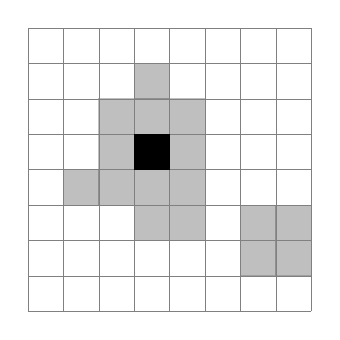
\begin{tikzpicture}[scale=0.45]
				\draw[help lines, step=1] (-4, -4) grid (4, 4);
				\foreach \x in {(-3, -1), (-2, -1), (-2, 0), (-2, 1), (-1, -2), (-1, -1), (-1, 0), (-1, 1), (-1, 2), (0, -2), (0, -1), (0, 0), (0, 1), (2, -3), (2, -2), (3, -3), (3, -2)}
				\filldraw[gray, opacity=0.5] \x rectangle + (1, 1);
				\foreach \x in {(-1, 0)}
				\filldraw[black] \x rectangle + (1, 1);
			\end{tikzpicture}
			\caption{Result of binary erosion of the image with a $3 \times 3$ pixel structuring element. The transparent pixels are now set to zero.}
		\end{subfigure}
	\end{figure}
\end{frame}
\begin{frame}{Example of binary morphological opening - 2/2}
	\begin{figure}
		\begin{subfigure}[t]{0.45\linewidth}
			\centering
			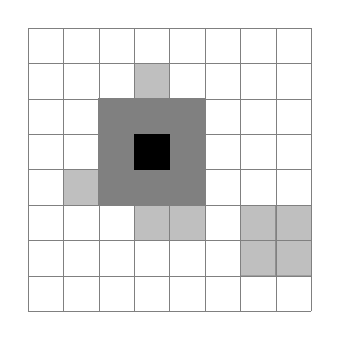
\begin{tikzpicture}[scale=0.45]
				\draw[help lines, step=1] (-4, -4) grid (4, 4);
				\foreach \x in {(-3, -1), (-1, -2), (-1, 2), (0, -2), (2, -3), (2, -2), (3, -3), (3, -2)}
				\filldraw[gray, opacity=0.5] \x rectangle + (1, 1);
				\foreach \x in {(-2, -1), (-2, 0), (-2, 1), (-1, -1), (-1, 0), (-1, 1), (0, -1), (0, 0), (0, 1)}
				\filldraw[gray] \x rectangle + (1, 1);
				\foreach \x in {(-1, 0)}
				\filldraw[black] \x rectangle + (1, 1);
			\end{tikzpicture}
			\caption{Image after binary opening, i.e. erosion and dilation. The gray pixels were set to one again.}
		\end{subfigure}
		\hfill
		\begin{subfigure}[t]{0.45\linewidth}
			\centering
			
\begin{tikzpicture}[scale=0.45]
				\draw[help lines, step=1] (-4, -4) grid (4, 4);
				\foreach \x in {(-2, -1), (-2, 0), (-2, 1), (-1, -1), (-1, 0), (-1, 1), (0, -1), (0, 0), (0, 1)}
				\filldraw[black] \x rectangle + (1, 1);
			\end{tikzpicture}
			\caption{Result of opening. Outliers have been eliminated and edges have been smoothed.}
		\end{subfigure}
	\end{figure}
\end{frame}

\begin{frame}{Example of binary morphological closing - 1/2}
	\begin{figure}
		\centering
		\begin{subfigure}[t]{0.45\linewidth}
			\centering
			
\begin{tikzpicture}[scale=0.45]
			\draw[help lines, step=1] (-4, -4) grid (4, 4);
			\foreach \x in {(-2, 0), (-2, 2), (1, 1), (1, -2)}
			\filldraw[black] \x rectangle + (1, 1);
			\end{tikzpicture}
			\caption{Binary image, where the pixels with value one are black.}
		\end{subfigure}
		\hfill
		\begin{subfigure}[t]{0.45\linewidth}
			\centering
			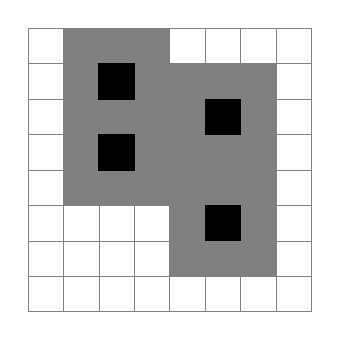
\begin{tikzpicture}[scale=0.45]
			\draw[help lines, step=1] (-4, -4) grid (4, 4);
			\foreach \x in {(-3, -1), (-3, 0), (-3, 1), (-3, 2), (-3, 3), (-2, -1), (-2, 0), (-2, 1), (-2, 2), (-2, 3), (-1, -1), (-1, 0), (-1, 1), (-1, 2), (-1, 3), (0, -3), (0, -2), (0, -1), (0, 0), (0, 1), (0, 2), (1, -3), (1, -2), (1, -1), (1, 0), (1, 1), (1, 2), (2, -3), (2, -2), (2, -1), (2, 0), (2, 1), (2, 2)}
			\filldraw[gray] \x rectangle + (1, 1);
			\foreach \x in {(-2, 0), (-2, 2), (1, 1), (1, -2)}
			\filldraw[black] \x rectangle + (1, 1);
			\end{tikzpicture}
			\caption{Image after binary dilation with a $3 \times 3$ pixel structuring element. The gray pixels are now set to one.}
		\end{subfigure}
	\end{figure}
\end{frame}
\begin{frame}{Example of binary morphological closing - 2/2}
	\begin{figure}
		\begin{subfigure}[t]{0.45\linewidth}
			\centering
			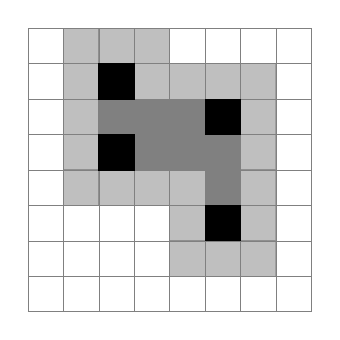
\begin{tikzpicture}[scale=0.45]
			\draw[help lines, step=1] (-4, -4) grid (4, 4);
			\foreach \x in {(-3, -1), (-3, 0), (-3, 1), (-3, 2), (-3, 3), (-2, -1), (-2, 3), (-1, -1), (-1, 2), (-1, 3), (0, -3), (0, -2), (0, -1), (0, 2), (1, -3), (1, 2), (2, -3), (2, -2), (2, -1), (2, 0), (2, 1), (2, 2)}
			\filldraw[gray, opacity=0.5] \x rectangle + (1, 1);
			\foreach \x in {(-2, 0), (-2, 1), (-2, 2), (-1, 0), (-1, 1), (0, 0), (0, 1), (1, -2), (1, -1), (1, 0), (1, 1)}
			\filldraw[gray] \x rectangle + (1, 1);
			\foreach \x in {(-2, 0), (-2, 2), (1, 1), (1, -2)}
			\filldraw[black] \x rectangle + (1, 1);
			\end{tikzpicture}
			\caption{Image after binary closing, i.e. dilation and erosion. The transparent pixels are set to zero again.}
		\end{subfigure}
		\hfill
		\begin{subfigure}[t]{0.45\linewidth}
			\centering
			
\begin{tikzpicture}[scale=0.45]
			\draw[help lines, step=1] (-4, -4) grid (4, 4);
			\foreach \x in {(-2, 0), (-2, 1), (-2, 2), (-1, 0), (-1, 1), (0, 0), (0, 1), (1, -2), (1, -1), (1, 0), (1, 1)}
			\filldraw[black] \x rectangle + (1, 1);
			\end{tikzpicture}
			\caption{Result of closing. The gaps between pixels have been filled.}
		\end{subfigure}
	\end{figure}
\end{frame}

\begin{frame}
	Notes on binary morphological opening \& closing:
	\begin{itemize}
		\item The outcome is highly dependent on the \emph{chosen} structuring element $\Psi \subseteq \mathbb{Z}^2$.
		\item Morphological opening smoothes edges and eliminates outliers.
		\item Morphological closing smoothes edges and fills gaps.
		\item $\mathfrak{I} \circ \Psi \subseteq \mathfrak{I} \subseteq \mathfrak{I} \bullet \Psi$
	\end{itemize}
\end{frame}

\begin{frame}
	\begin{lemma}
		Let $m, n \in \mathbb{N}$ and $\Psi \subseteq \mathbb{Z}^2$ be a structuring element. Let $(i, j) \in \Omega$. Then the following equalities hold:
		\begin{equation*}
			\begin{aligned}
				\big\{ \mathfrak{I} &\in \{ 0, 1 \}^{m \times n} \mid (\mathfrak{I} \circ \Psi)(i, j) = 1 \big\} \\
				&= \bigcup_{(k, l) \in \Psi} \bigcap_{(\tilde{k}, \tilde{l}) \in \Psi} \left\{ \mathfrak{I} \in \{ 0, 1 \}^{m \times n} \mid \mathfrak{I}(i - k + \tilde{k}, j - l + \tilde{l}) = 1 \right\}
			\end{aligned}
		\end{equation*}
		\begin{equation*}
			\begin{aligned}
				\big\{ \mathfrak{I} &\in \{ 0, 1 \}^{m \times n} \mid (\mathfrak{I} \bullet \Psi)(i, j) = 1 \big\} \\
				&= \bigcap_{(k, l) \in \Psi} \bigcup_{(\tilde{k}, \tilde{l}) \in \Psi} \left\{ \mathfrak{I} \in \{ 0, 1 \}^{m \times n} \mid \mathfrak{I}(i + k - \tilde{k}, j + l - \tilde{l}) = 1 \right\}
			\end{aligned}
		\end{equation*}
	\end{lemma}
\end{frame}

\subsection{Main results: Changes of the error probabilities after morphological opening \& closing}

\begin{frame}
	\begin{beamercolorbox}[sep=8pt,center,shadow=true,rounded=true]{title}
		Question: What is the effect of opening and closing on the probabilities of a type I and II error?
	\end{beamercolorbox}
\end{frame}

\begin{frame}
	\begin{theorem}
		Let $\alpha \in (0, 1)$ and $t_\alpha$ a threshold, such that
		\begin{equation*}
			\min \left\{ \mathbb{P}_V\left( \norm{\Delta^+ F(i, j)} \geq t_\alpha \right), \mathbb{P}_V\left( \norm{\Delta^- F(i, j)} \geq t_\alpha \right) \right\} \leq \alpha
		\end{equation*}
		for all $V \in \mathcal{H}_0(i, j)$. \pause Let $\mathfrak{I}_\alpha$ be the binary image defined by
		\begin{equation*}
			\mathfrak{I}_\alpha(i, j) = \mathds{1}_{ \{ T(i, j) \geq t_\alpha \} }
		\end{equation*}
		for all $(i, j) \in \Omega$. \pause
		
		Let $\varphi \in \mathbb{N}$ be odd. Let $\Phi_\varphi = \left\{ -\frac{\varphi - 1}{2}, -\frac{\varphi - 3}{2}, \dots, \frac{\varphi - 3}{2}, \frac{\varphi - 1}{2} \right\}$ and $\Psi_\varphi = \Phi_\varphi \times \Phi_\varphi$ be a structuring element. Let $(i, j) \in \Omega$ and $V \in \mathcal{H}_0(i, j)$. \pause
		Then the following inequalities hold:
		\begin{align}
			\mathbb{P}_V\left( (\mathfrak{I}_\alpha \circ \Psi_\varphi)(i, j) = 1 \right) &\leq \varphi \alpha^{\frac{\varphi + 1}{2}} \\
			\mathbb{P}_V\left( ((\mathfrak{I}_\alpha \circ \Psi_\varphi) \bullet \Psi_\varphi)(i, j) = 1 \right) &\leq \varphi^3 \alpha^{\frac{\varphi + 1}{2}}
		\end{align}
	\end{theorem}
\end{frame}

\begin{frame}
	Main ideas of the proof:
	\begin{itemize}
		\item Note, that if $H_0(i, j)$ is true, then the null hypothesis is true for a whole row or column in the image.
		\item If we only take every second pixel in the row/column, they will be independent, which yields the exponent $\frac{\varphi + 1}{2}$.
	\end{itemize}
\end{frame}

\begin{frame}
	\begin{figure}
		\centering
		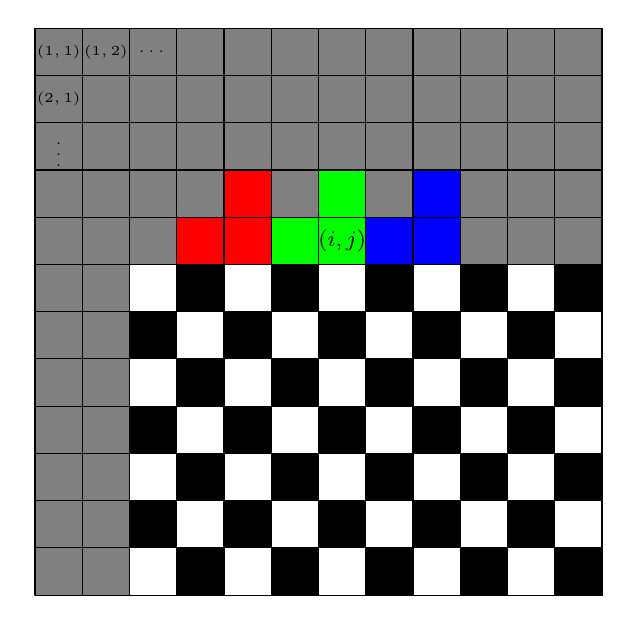
\begin{tikzpicture}[scale=0.6]
			\foreach \i in {-6, ..., 5}
				\foreach \j in {-6, ..., 5}
					\filldraw[gray] (\i, \j) rectangle + (1, 1);
			\foreach \i in {-4, ..., 5}
				\foreach \j in {-6, ..., 0}
				{
					\pgfmathparse{mod(\i+\j, 2) ? "black" : "white"}
					\edef\colour{\pgfmathresult}
					\filldraw[fill=\colour] (\i, \j) rectangle + (1, 1);
				}
			\foreach \x in {(-2, 1), (-3, 1), (-2, 2)}
				\filldraw[red] \x rectangle + (1, 1);
			\foreach \x in {(0, 1), (-1, 1), (0, 2)}
				\filldraw[green] \x rectangle + (1, 1);
			\foreach \x in {(2, 1), (1, 1), (2, 2)}
				\filldraw[blue] \x rectangle + (1, 1);
			\draw[step=1] (-6, -6) grid (6, 6);
			\node at (0.5, 1.5) {\footnotesize $(i, j)$};
			\node at (-5.5, 5.5) {\tiny $(1, 1)$};
			\node at (-4.5, 5.5) {\tiny $(1, 2)$};
			\node at (-3.5, 5.5) {\tiny $\dots$};
			\node at (-5.5, 4.5) {\tiny $(2, 1)$};
			\node at (-5.5, 3.5) {\tiny $\vdots$};
		\end{tikzpicture}
		\caption{The random variable $\norm{\Delta^- F(i, j)}$ only depends on the green pixels, $\norm{\Delta^- F(i, j - 2)}$ depends on the red pixels and $\norm{\Delta^- F(i, j + 2)}$ on the blue pixels. Since these are all distinct from another, the random variables are independent.}
	\end{figure}
\end{frame}






\begin{frame}
	\begin{theorem}
		Let $t$ be a threshold, such that
		\begin{equation*}
			\mathbb{P}_V\left( T(i, j) \leq t \right) \leq \beta
		\end{equation*}
		for all $V \in \mathcal{H}_1(i, j)$. \pause Let $\mathfrak{I}$ be the binary image defined by
		\begin{equation*}
			\mathfrak{I}(i, j) = \mathds{1}_{ \{ T(i, j) \geq t \} }
		\end{equation*}
		for all $(i, j) \in \Omega$. \pause
		
		Let $\varphi \in \mathbb{N}$ be odd. Let $\Phi_\varphi = \{ -\frac{\varphi - 1}{2}, -\frac{\varphi - 3}{2}, \dots, \frac{\varphi - 3}{2}, \frac{\varphi - 1}{2} \}$ and $\Psi_\varphi = \Phi_\varphi \times \Phi_\varphi$ be a structuring element. Let $(i, j) \in \Omega$ and $V \in \mathcal{H}_1(i, j)$. \pause
		
		Denote by $\varLambda = \{ \kappa_1, \dots, \kappa_2 \} \times \{ \lambda_1, \dots, \lambda_2 \}$ the rROI contained in $V$. Let $\min \{ \kappa_2 - \kappa_1 + 1, \lambda_2 - \lambda_1 + 1 \} \geq \varphi$. \pause
		Then the following inequalities hold:
		\begin{align}
			\mathbb{P}_V\left( (\mathfrak{I} \circ \Psi_\varphi)(i, j) = 0 \right) &\leq \varphi^2 \beta \\
			\mathbb{P}_V\left( ((\mathfrak{I} \circ \Psi_\varphi) \bullet \Psi_\varphi)(i, j) = 0 \right) &\leq \varphi^2 \beta
		\end{align}
	\end{theorem}
\end{frame}

\begin{frame}
	Main ideas of the proof:
	\begin{itemize}
		\item Note, that if $H_0(i, j)$ is true, then there exists a square with side length $\varphi$, such that the null hypothesis is true for every pixel inside that square.
		\item The square has $\varphi^2$ pixels and for each pixel the probability of a type II error is less than $\beta$.
	\end{itemize}
	
	Note: We expect a lower probability than $\varphi^2 \beta$ after opening and closing. This does not seem provable with the methods used, since any independence is gone after opening. The expected improvement through closing can be observed in the numerical results.
\end{frame}

\subsection{Numerical results}

\begin{frame}{Methodology}
	\begin{itemize}
		\item Create 5 test images each for $128 \times 128$, $256 \times 256$ and $512 \times 512$ pixel.
		\item Determine the correct region of interest.
		\item Perform the following 50 times to even out outliers:
		\begin{itemize}
			\item Create standard normal distributed noise.
			\item Loop over the standard deviation $\sigma \in \{ 1, \dots, 150 \}$ and add the noise multiplied by the standard deviation to the image.
			\begin{itemize}
				\item Binarize the image using the testing procedure from the first section with $\alpha = 0.05$ and $t_{0.05} = 3.2555 \sigma$.
				\item Perform binary morphological opening.
				\item Perform binary morphological closing.
			\end{itemize}
			\item In each step, count the number of type I and II errors for each $\sigma$ separately.
		\end{itemize}
		\item Add up all type I and II errors for all images and divide by the total number of background/foreground pixel, respectively.
	\end{itemize}
\end{frame}

\begin{frame}
	\begin{figure}
		\centering
		\begin{tikzpicture}[scale=0.8]
			\begin{axis}[
				legend pos=north west,
				xlabel=Standard deviation $\sigma$,
				ylabel=Proportion of type I errors,
				grid=both,
				minor grid style={gray!25},
				major grid style={gray!25},
				ymin=-0.05,
				ymax=1.05,
				width=\linewidth,
				no marks]
				\addplot[line width=1pt,color=blue] table[x=sigma,y=probtypeI,col sep=comma]{CSV/resultsErrorTestCasesTypeI.csv};
				\addlegendentry{Binarization}
				\addplot[line width=1pt,color=red] table[x=sigma,y=probtypeI,col sep=comma]{CSV/resultsErrorTestCasesTypeI_o.csv};
				\addlegendentry{Opening}
				\addplot[line width=1pt,color=gray] table[x=sigma,y=probtypeI,col sep=comma]{CSV/resultsErrorTestCasesTypeI_oc.csv};
				\addlegendentry{Opening \& Closing}
			\end{axis}
		\end{tikzpicture}
		\caption{Proportion of type I errors after binarization, opening and closing.}
	\end{figure}
\end{frame}
\begin{frame}
	\begin{figure}
		\begin{tikzpicture}[scale=0.8]
			\begin{axis}[
				legend pos=north west,
				xlabel=Standard deviation $\sigma$,
				ylabel=Proportion of type II errors,
				grid=both,
				minor grid style={gray!25},
				major grid style={gray!25},
				ymin=-0.05,
				ymax=1.05,
				width=\linewidth,
				no marks]
				\addplot[line width=1pt,color=blue] table[x=sigma,y=probtypeII,col sep=comma]{CSV/resultsErrorTestCasesTypeII.csv};
				\addlegendentry{Binarization}
				\addplot[line width=1pt,color=red] table[x=sigma,y=probtypeII,col sep=comma]{CSV/resultsErrorTestCasesTypeII_o.csv};
				\addlegendentry{Opening}
				\addplot[line width=1pt,color=gray] table[x=sigma,y=probtypeII,col sep=comma]{CSV/resultsErrorTestCasesTypeII_oc.csv};
				\addlegendentry{Opening \& Closing}
			\end{axis}
		\end{tikzpicture}
		\caption{Proportion of type II errors after binarization, opening and closing.}
	\end{figure}
\end{frame}

\section{Outlook}

\begin{frame}
	\begin{block}{How did we obtain the exponent $\frac{\varphi + 1}{2}$?}
		For a background pixel to be falsely identified as foreground after opening, at least $\frac{\varphi + 1}{2}$ many pixels background pixels have to be falsely categorized by the binarization through the statistical test. This is the \emph{minimum number of independent points in a structuring element} that can lead to a false categorization of a pixel. With this connection in mind, the techniques to prove the main results of this paper might present themselves useful in other cases as well.
	\end{block}
	\pause
	\begin{block}{What can be gained by using multiple testing techniques?}
		The main results of this work only considered the categorization of a single pixel. Since we perform tests for all pixels at once, the analysis of techniques from multiple testing in connection with morphological operations would be an interesting field of study to expand the results of this paper.
	\end{block}
\end{frame}

\begin{frame}
	\centering
	Thank you for the attention!
\end{frame}


\end{document}
